\setcounter{page}{1} \pagenumbering{Alph}

% Add PDF bookmark 
\pdfbookmark[0]{Title}{Title}

\thispagestyle{empty}
\begin{flushleft} ~\\ \vspace{-10mm} \hspace{-9mm}  
\includegraphics[width=90mm, height=23mm]{Cover/istlogo} \hspace{49mm}  \includegraphics[height=23mm]{Cover/fml} 
\\ \vspace{5mm}
%~\\ \vspace{50mm} % gr�ficos
~\\ \begin{center} 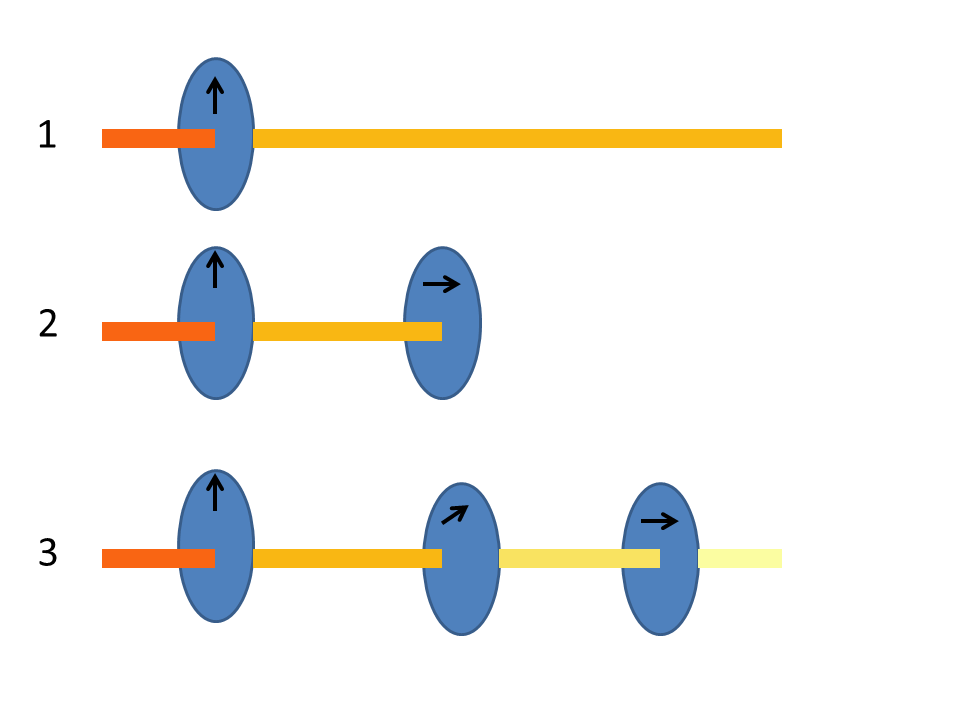
\includegraphics[height=50mm]{Cover/coverimage}  \end{center} % gr�ficos
~\\ \vspace{5mm}
\begin{centering}
\LARGE \textbf{Fancy Title 1}
\\ \vspace{5mm}
\Large Fancy Subtitle 1
\\ \vspace{15mm}
\Large \textbf{Full Name} \\
(Licenciado)
\\ \vspace{15mm}
\Large Disserta��o para obter o grau de Mestre em
\\ \vspace{2mm}
\LARGE \textbf{Engenharia Biom�dica}
\\ \vspace{20mm}

\Large \textbf{J�ri}

\begin{tabular}{lcl}
\large Presidente:		&   & \large \\ 
\large Orientador: 		&   & \large \\ 
\large Co-Orientador: &   & \large \\ 
\large Vogal:	 				&   & \large \\
\end{tabular}
 
\vspace{9mm}

%\Large \textbf{\todaythesis\today} \\
\Large \textbf{Janeiro 2012} \\
\end{centering}
\let\thepage\relax
\end{flushleft}
\pagebreak


\clearpage
% Since I am using double sided pages, the second page should be white.
% Remember that when delivering the dissertation, IST requires for the cover to appear twice.

\thispagestyle{empty}
\cleardoublepage

\setcounter{page}{1} \pagenumbering{roman}

\baselineskip 18pt % line spacing: -12pt for single spacing
                   %               -18pt for 1 1/2 spacing
                   %               -24pt for double spacingnts}